\section{Programación Matemática}

% --- El texto de la sección permanece igual ---
% Se usan los mismos comandos~\cite{key} y~\cite[page]{key}

El concepto de Programación Matemática\footnote{\textbf{Programación Matemática:} Rama de las matemáticas aplicadas que se ocupa de la teoría y los métodos para resolver problemas de optimización, es decir, encontrar el mejor valor (máximo o mínimo) de una función objetivo sujeta a un conjunto de restricciones.} constituye una disciplina fundamental y contemporánea dentro del campo de las Matemáticas Aplicadas. Se define como el área dedicada al estudio y desarrollo de la teoría, los algoritmos y las aplicaciones para la resolución de problemas de optimización, donde se busca seleccionar la mejor alternativa entre un conjunto de opciones disponibles, sujeta a un conjunto de restricciones~\cite[p.~1]{sinha2006},~\cite[p.~1]{luenberger1984}. En esencia, la Programación Matemática se enfoca en la identificación y determinación de la solución más ventajosa o eficiente para un problema específico, considerando un conjunto predefinido de restricciones que delinean el espacio de alternativas factibles~\cite[p.~1]{sinha2006}. La optimización, por lo tanto, se erige como el núcleo central de la Programación Matemática, buscando la asignación más efectiva de recursos escasos para alcanzar objetivos concretos.\ \textit{Management Science}\footnote{\textbf{Management Science (Ciencia de la Gestión):} Disciplina que utiliza un enfoque científico, a menudo cuantitativo, para la toma de decisiones gerenciales y la resolución de problemas en organizaciones.} (Ciencia de la Gestión), una disciplina caracterizada por un enfoque científico para la toma de decisiones gerenciales, utiliza la Programación Matemática como una de sus herramientas más poderosas, aplicando métodos matemáticos y las capacidades de las computadoras modernas a los problemas complejos y no estructurados que enfrentan los gestores~\cite[p.~1]{bradley1977applied}.

Desde una perspectiva formal, la Programación Matemática implica la formulación de una representación abstracta del problema a través de un modelo matemático, seguido por la aplicación de algoritmos de optimización para la determinación de los valores óptimos que deben adoptar las variables de decisión dentro de dicho modelo~\cite[p.~175]{bertsekas1999}. Un problema de optimización general se puede plantear como la selección de variables de decisión $x_1, x_2, \ldots, x_n$ de una región factible dada, de tal manera que se optimice (minimice o maximice) una función objetivo $f(x_1, x_2, \ldots, x_n)$~\cite[p.~410]{nocedal2006}.

Los principios fundamentales de la Programación Matemática se estructuran en torno a los componentes esenciales que definen cualquier problema de optimización. Estos incluyen:
\begin{enumerate}
    \item \textbf{Variables de Decisión:} Cantidades que el tomador de decisiones controla y cuyos valores determinan la solución del modelo~\cite[p.~181]{bradley1977applied}.
    \item \textbf{Función Objetivo:} Una medida de rendimiento o efectividad, expresada como una función matemática de las variables de decisión, que se busca maximizar o minimizar~\cite[p.~181]{bradley1977applied}.
    \item \textbf{Restricciones:} Un conjunto de relaciones (ecuaciones o inecuaciones) que las variables de decisión deben satisfacer, reflejando las limitaciones impuestas por la naturaleza del problema (disponibilidad de recursos, requisitos tecnológicos, etc.)~\cite[p.~181]{bradley1977applied}.
\end{enumerate}

El objetivo primordial es, por lo tanto, determinar los valores óptimos de las variables de decisión que no solo satisfacen todas las restricciones impuestas al sistema, sino que también logran el mejor valor posible para la función objetivo.

El desarrollo formal de la Programación Matemática, especialmente la Programación Lineal, se consolidó a mediados del siglo XX.\ George B. Dantzig es ampliamente reconocido por el desarrollo del \textit{algoritmo simplex} alrededor de 1947, que proporcionó un método sistemático y eficiente para resolver problemas de Programación Lineal~\cite[p.~2]{sinha2006},~\cite[p.~1]{bradley1977applied}. Este avance fue un punto de inflexión, impulsado en gran medida por la necesidad de optimizar la asignación de recursos durante la Segunda Guerra Mundial en el contexto de la \textit{Investigación Operativa}\footnote{\textbf{Investigación Operativa (Operations Research):} Disciplina que aplica métodos analíticos avanzados para ayudar a tomar mejores decisiones. Surgió durante la Segunda Guerra Mundial para resolver problemas militares complejos.} (Operations Research)~\cite[p.~1]{sinha2006}. Sin embargo, los fundamentos de la optimización se pueden rastrear a trabajos mucho anteriores de matemáticos como Lagrange y Fourier~\cite[p.~1]{sinha2006}. En la década de 1950, surgieron avances significativos en Programación No Lineal con las contribuciones de Kuhn y Tucker sobre condiciones de optimalidad, y en Programación Dinámica gracias a Richard Bellman~\cite[p.~9]{sinha2006}. Ralph Gomory realizó trabajos pioneros en Programación Entera durante el mismo período~\cite[p.~9]{sinha2006}.

\subsection{Variantes Principales de la Programación Matemática}

La Programación Matemática abarca diversas variantes, cada una diseñada para tipos específicos de problemas:

\begin{enumerate}[label=\arabic*.]
    \item \textbf{Programación Lineal (PL):}
    Se caracteriza porque tanto la función objetivo como todas las restricciones son funciones lineales de las variables de decisión~\cite[p.~2]{sinha2006},~\cite[p.~9]{bradley1977applied}. Los principios fundamentales de la PL incluyen la proporcionalidad (la contribución de cada variable es proporcional a su valor), la aditividad (la contribución total es la suma de las contribuciones individuales), la divisibilidad (las variables pueden tomar valores fraccionarios) y la certeza (todos los parámetros del modelo son conocidos con exactitud)~\cite[p.~9]{bradley1977applied}. La forma general de un problema de PL es: \\
    Optimizar $z = \sum_{j=1}^{n} c_j x_j$ \\
    Sujeto a:
    \begin{align*}
        \sum_{j=1}^{n} a_{ij} x_j & (\leq, =, \geq) b_i, && \text{para } i = 1, \ldots, m_1+m_2+m_3 \\
        x_j & \geq 0 && \text{(para algunas o todas las } j\text{)} \\ %chktex 9
        x_j & \text{ irrestricta} && \text{(para algunas o todas las } j\text{)} %chktex 9
    \end{align*}
~\cite[p.~117]{sinha2006}. \\
    \begin{figure}
        \centering
        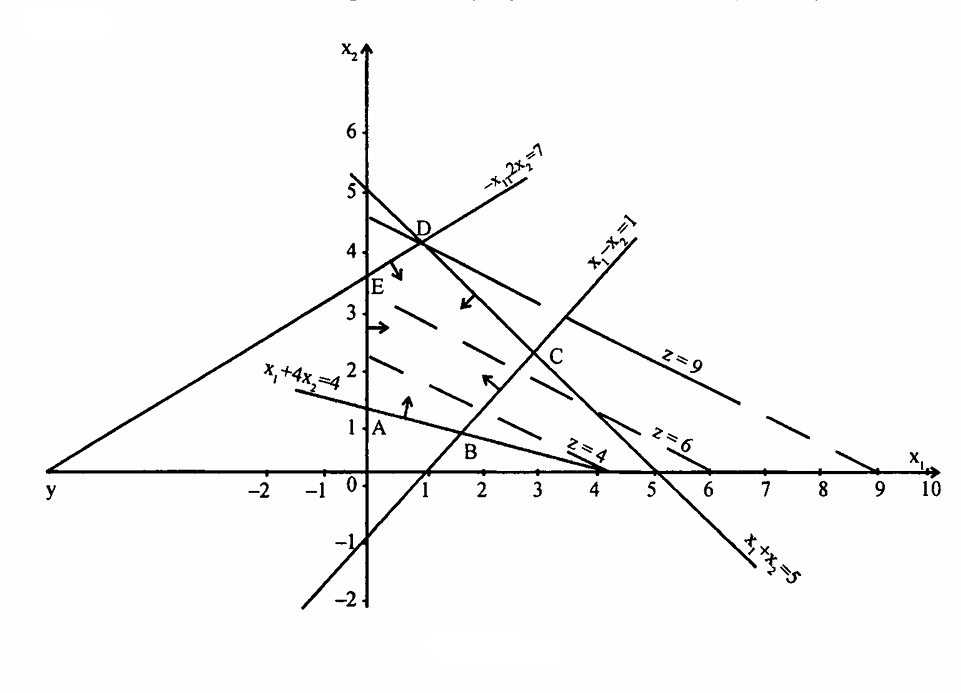
\includegraphics[width=0.75\linewidth]{img/marcoTeorico/mathprogramming_fig1.png}
        \caption{Representación bidimensional de la región factible de un problema de programación lineal, caracterizada por un polígono convexo definido por restricciones lineales. Se incluyen líneas de nivel de la función objetivo y el punto óptimo ubicado en un vértice del conjunto factible, ilustrando la solución típica en problemas lineales. Adaptado de~\cite[p.~6-7]{sinha2006}}%
        \label{fig:mathprogramming01}
    \end{figure}

    \item \textbf{Programación No Lineal (PNL):}
    Se aplica cuando la función objetivo o al menos una de las restricciones (o ambas) es una función no lineal de las variables de decisión~\cite[p.~9]{sinha2006},~\cite[p.~410]{nocedal2006}. A diferencia de la PL, donde el óptimo (si existe) se encuentra en un vértice de la región factible, en PNL el óptimo puede estar en el interior de la región, en su frontera (no necesariamente un vértice), o en un vértice~\cite[p.~413, Figura 13.1]{nocedal2006}. Una distinción crucial en PNL es entre óptimos locales y globales. Un óptimo local es una solución mejor que todas las soluciones ``cercanas'', mientras que un óptimo global es la mejor solución en toda la región factible~\cite[p.~413]{nocedal2006}. \\

    \begin{figure}
        \centering
        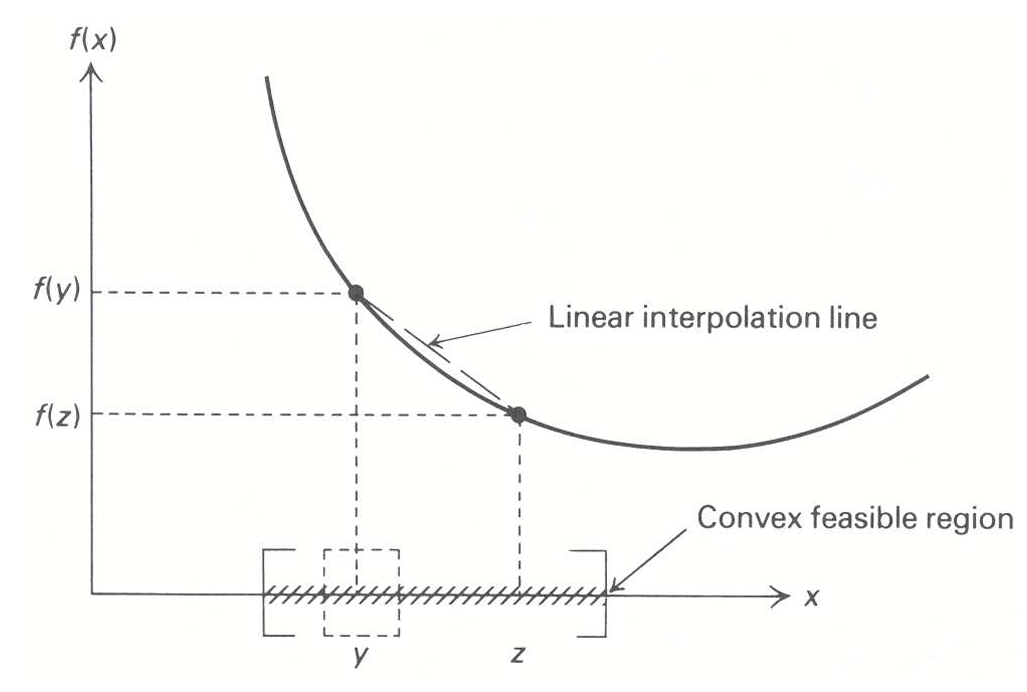
\includegraphics[width=0.75\linewidth]{img/marcoTeorico/mathprogramming_fig2.png}
        \caption{Visualización de una función no lineal con múltiples extremos locales y un único óptimo global, empleada para ilustrar las diferencias conceptuales entre mínimos (o máximos) locales y globales en problemas de programación no lineal. Esta distinción es clave en el análisis de algoritmos de optimización y su convergencia. Adaptado de~\cite[p.~419]{bradley1977applied}}%
        \label{fig:mathprogramming02}
    \end{figure}

    Dentro de la PNL, la \textit{Programación Convexa} es de particular importancia. Si un problema de minimización involucra minimizar una función convexa sobre un conjunto convexo, o un problema de maximización implica maximizar una función cóncava sobre un conjunto convexo, entonces cualquier óptimo local es también un óptimo global~\cite[p.~418]{nocedal2006},~\cite[p.~1]{boyd2004}.
    \begin{itemize}
        \item \textbf{Programación Cuadrática:} Un caso especial de PNL donde la función objetivo es cuadrática y las restricciones son lineales~\cite[p.~419]{nocedal2006}. Su forma general es: \\
        Maximizar $f(x) = \sum_{j=1}^{n} c_j x_j + \frac{1}{2} \sum_{j=1}^{n} \sum_{k=1}^{n} q_{jk} x_j x_k$ \\
        Sujeto a:
        \begin{align*}
            \sum_{j=1}^{n} a_{ij} x_j & \leq b_i, && \text{para } i = 1, \ldots, m \\
            x_j & \geq 0, && \text{para } j = 1, \ldots, n
        \end{align*}~\cite[p.~433]{nocedal2006}.
    \end{itemize}

    \item \textbf{Programación Entera (PE):}
    Se caracteriza porque algunas o todas las variables de decisión están restringidas a tomar valores enteros~\cite[p.~9]{sinha2006},~\cite[p.~272]{bradley1977pe}. Si todas las variables son enteras, se denomina \textit{Programación Entera Pura}; si solo algunas lo son, es \textit{Programación Entera Mixta}. Un caso especial importante es la \textit{Programación Binaria} o \textit{Programación 0\-1}, donde las variables solo pueden tomar los valores 0 o 1, útil para modelar decisiones de tipo sí/no (go/no-go)~\cite[p.~273]{bradley1977pe}. \\

    \item \textbf{Programación Dinámica (PD):}
    Es un enfoque que transforma un problema complejo en una secuencia de subproblemas más simples, interrelacionados. Su característica esencial es la naturaleza multietapa del procedimiento de optimización~\cite[p.~320]{bradley1977pd}. Se basa en el \textit{Principio de Optimalidad de Bellman}: una política óptima tiene la propiedad de que, cualesquiera que sean el estado y la decisión iniciales, las decisiones restantes deben constituir una política óptima con respecto al estado resultante de la primera decisión~\cite[p.~323]{bradley1977pd}. La PD utiliza ecuaciones recursivas para relacionar la solución óptima de un problema de $n$ etapas con la de un problema de $(n-1)$ etapas~\cite[p.~325]{bradley1977pd}.

    \item \textbf{Programación Estocástica:}
    Aborda problemas de optimización donde algunos de los parámetros del modelo (coeficientes de la función objetivo, lado derecho de las restricciones o coeficientes tecnológicos) son inciertos y se representan como variables aleatorias con distribuciones de probabilidad conocidas~\cite[p.~432]{sinha2006}. Los enfoques incluyen la optimización del valor esperado o la incorporación de restricciones probabilísticas (chance constraints).
\end{enumerate}


\subsection{Aplicaciones Típicas}

La Programación Matemática se aplica extensamente en diversos campos:
\begin{itemize}
    \item \textbf{Investigación Operativa:} Planificación de la producción, gestión de inventarios, problemas de transporte y asignación, secuenciación de tareas, optimización de rutas~\cite[p.~3-5]{sinha2006},~\cite[p.~1-2]{bradley1977applied}.
    \item \textbf{Economía y Finanzas:} Optimización de portafolios de inversión, asignación de capital, modelos de equilibrio económico, planificación del desarrollo económico~\cite[p.~100-102]{bradley1977applied},~\cite[p.~411]{nocedal2006}.
    \item \textbf{Ingeniería:} Diseño óptimo de estructuras, planificación de recursos hídricos, optimización de procesos químicos, problemas de carga de redes eléctricas~\cite[p.~412]{nocedal2006}.
    \item \textbf{Logística:} Localización de almacenes, diseño de redes de distribución, gestión de cadenas de suministro~\cite[p.~274]{bradley1977pe}.
\end{itemize}

En el ámbito de la física computacional y la simulación, aunque el término no siempre se use explícitamente, la optimización es fundamental. Por ejemplo, en la minimización de energía en sistemas moleculares, la optimización de parámetros en modelos físicos, o la búsqueda de configuraciones óptimas en simulaciones de N-cuerpos. Los métodos de Programación Matemática, como la Programación Cuadrática, son relevantes para problemas de ajuste de curvas (regresión restringida) en el análisis de datos experimentales~\cite[p.~412]{nocedal2006}.

\subsection{Ventajas y Desventajas}

\begin{itemize}
    \item \textbf{Ventajas:}
    \begin{itemize}
        \item Proporciona un marco estructurado para la toma de decisiones y la optimización de recursos limitados~\cite[p.~182]{bradley1977applied}.
        \item Permite modelar sistemas complejos y encontrar soluciones óptimas o cercanas a la óptima que pueden no ser intuitivas~\cite[p.~183]{bradley1977applied}.
        \item La teoría de la dualidad y el análisis de sensibilidad ofrecen información valiosa sobre el valor de los recursos (precios sombra) y la robustez de la solución ante cambios en los parámetros del modelo~\cite[p.~78-91]{bradley1977applied}.
        \item La disponibilidad de software eficiente permite resolver problemas de gran escala, especialmente en Programación Lineal~\cite[p.~182]{bradley1977applied}.
    \end{itemize}

    \item \textbf{Desventajas/Limitaciones:}
    \begin{itemize}
        \item La formulación de un modelo matemático preciso puede ser compleja y consumir mucho tiempo, requiriendo una comprensión profunda del problema y de las técnicas de modelado~\cite[p.~183]{bradley1977applied}.
        \item Para problemas no lineales no convexos, los algoritmos pueden converger a óptimos locales en lugar de globales~\cite[p.~413]{nocedal2006}.
        \item La Programación Entera, especialmente para problemas grandes, puede ser computacionalmente muy demandante (``NP-hard'')~\cite[p.~287]{bradley1977pe}.
        \item La suposición de certeza en los parámetros (en modelos determinísticos) puede no reflejar la realidad; aunque la Programación Estocástica aborda esto, incrementa la complejidad del modelo~\cite[p.~432]{sinha2006}.
        \item La calidad de la solución depende críticamente de la calidad y disponibilidad de los datos~\cite[p.~183]{bradley1977applied}.
    \end{itemize}
\end{itemize}
